% !TEX program = xelatex
%
% Distillation and reinforcement learning for Macedonian poetic style
% transfer: SFT and GRPO (v1, v2) of a Qwen3-4B student. Split out of
% report.tex. Compile with `xelatex rl_report.tex` (native Cyrillic via
% fontspec/polyglossia), not pdflatex. The Gemma 4 E4B student is reported
% separately once trained.
\documentclass[11pt]{article}

\usepackage{fontspec}
\usepackage{polyglossia}
\setmainlanguage{english}
\setotherlanguage{macedonian}
\setmainfont{Times New Roman}
\setmonofont{Courier New}
\newfontfamily\cyrillicfont{Times New Roman}
\usepackage{amsmath}
\usepackage{booktabs}
\usepackage{graphicx}
\usepackage{hyperref}
\usepackage{geometry}
\geometry{margin=2.3cm}
\sloppy

\title{Distilling and Reinforcing Macedonian Poetic Style Transfer:\\
SFT and GRPO on a 4B Student}
\date{\today}

\begin{document}
\maketitle

\begin{abstract}
Gemma~4 31B, given a heavily scaffolded prompt (author style profile,
vocabulary palette, exemplar lines, structural targets), rewrites a Macedonian
poem in a named poet's style. We distil this into Qwen3-4B given only the
source poem and the target author's name: LoRA supervised fine-tuning (SFT) on
1{,}146 teacher outputs, then Group Relative Policy Optimization (GRPO) against
a reward built from the project's stylometric profiles, line-level content
similarity and gates against copying, repetition and malformed output. SFT
teaches the task format completely but collapses ten voices into one dominated
by the corpus's two largest authors. GRPO-v1 raises the reward from 0.254 to
0.406, removes SFT's repetition and doubles content preservation, but lowers
author identification and learns to copy single source lines. GRPO-v2, which
reweights the classifier term and steepens the copy gate, keeps identification
near the SFT level only by holding the policy on the two largest authors. For
eight of the ten targets neither student is ever identified as the requested
author, which leaves GRPO's group-relative update nothing to amplify. All
results are on the validation split; the test-split run is in progress.
\end{abstract}

% ═══════════════════════════════════════════════════════════════════════════
\section{Setup}\label{sec:setup}

\paragraph{Task.} \emph{source poem} $+$ \emph{target author's name}
$\to$ \emph{new poem} in the target's voice, in Macedonian Cyrillic. The
teacher (Gemma~4 31B behind a rate-limited API, about three minutes per poem
including obligatory reasoning) needs the whole stylometric pipeline at
inference time; the student needs none of it.

\paragraph{Data.} \texttt{make\_splits.py} splits the 1{,}239 poems of the 38
profiled authors 80/10/10 per author (seed 42) into 987 train, 126 val and 126
test poems; the unit is the poem, since (author, title) is not unique in the
corpus. The ten target authors are the ten with the most poems: Блаже
Конески, Пијан Славеј, Ефтим Клетников, Ристо Лазаров, Веле Смилевски,
Братислав Ташковски, Влада Урошевиќ, Адем Гајтани, Славко Јаневски and
Катица Ќулавкова. The teacher wrote 1{,}146 transfers for (train poem,
target) pairs, 108--120 per target, reusing the same 130 source poems across
targets so that the data contrasts authors on identical content.

\paragraph{Evaluation.} Every system is generated for the same 468 val pairs
(50 val poems $\times$ 10 targets, self pairs skipped), with the same prompt,
per-item seeds and plain sampling ($T=0.7$, top-$p=0.9$, top-$k=20$, 512 new
tokens), on one A100. The teacher was run on the same 468 pairs as a
reference. Metrics (\texttt{style\_metrics.py}) are all higher-is-better and
shared with the GRPO reward:
\begin{itemize}\itemsep0pt
  \item \emph{degeneracy}: distinct-$n$, line uniqueness; an output is
    \emph{degenerate} if distinct-1 $<0.40$ or line uniqueness $<0.80$;
  \item \emph{copying}: \emph{line novelty} (share of lines not verbatim from
    the source) and \emph{copy novelty} (share not near-copies; \S\ref{sec:reward});
  \item \emph{content}: content-word recall from the source;
  \item \emph{target style}: structural fit, TF-IDF palette hit rate, and two
    author classifiers. The reward classifier (\texttt{classifier.pkl},
    character 2--4-grams, linear SVM) was fitted on the whole corpus, so it
    memorises real poems (top-1 1.000 against 0.883 under 5-fold CV), and it
    is a GRPO reward term. The \emph{judge} is evaluation-only and differs on
    every axis: train poems only, word uni+bigrams, logistic regression. Its
    top-1 on unseen real poems of the ten targets is 0.663, the ceiling for a
    perfect transfer.
\end{itemize}

% ═══════════════════════════════════════════════════════════════════════════
\section{Supervised fine-tuning}\label{sec:sft}

The student sees a minimal chat: a one-sentence system instruction, the source
poem and the target's name, and the teacher's poem as the answer. None of the
teacher's scaffolding is in the prompt; whatever it knows about an author it
learns from about 115 teacher poems. One module (\texttt{sft\_data.py})
renders the prompt for training, evaluation and GRPO, so they cannot drift.
LoRA (rank 16, $\alpha$ 32, dropout 0.05) on all attention and MLP projections
of \texttt{Qwen/Qwen3-4B}; 3 epochs, effective batch 16, learning rate
$2\times10^{-4}$ (cosine), max length 1024, bf16, loss on the assistant turn
only. The run took 210 steps and 15 minutes on one A100. Loss fell from 2.87
to 1.72 in the first epoch and to 1.34 by the third, with steps at the epoch
boundaries that suggest partial memorisation of the training poems. 71
examples (6.2\,\%) are longer than 1024 tokens and lost their end-of-turn
token; SFT was not retrained, to keep both GRPO runs' start policy fixed.

\paragraph{Result.} Against the untuned base (Table~\ref{tab:main}), SFT
does the task: the base model mostly reproduces the source under a markdown
heading (line novelty 0.224, markup-free in 59\,\% of outputs), while SFT
writes original lines (1.000), never adds markup or commentary, fits the
target's structure (0.846 vs.\ 0.680), and is identified as the target 17
times more often (classifier top-1 0.158 vs.\ 0.009; judge 0.158 vs.\ 0.064).
The base model's higher content recall (0.901) and diversity come from the
copied human text.

\paragraph{Two deficits.} \emph{Style collapse}: the aggregate is carried by
Конески and Пијан Славеј, the corpus's two largest authors; the other eight
targets are identified 0--15\,\% of the time (Table~\ref{tab:authors}), and
36\,\% of all outputs are read as Конески whatever the target. The training
data is balanced across targets, so the imbalance is not one of example
counts. Pooled vocabulary at a matched 30{,}000-token budget is 3{,}087 word
types, against 5{,}376 for the teacher and 9{,}060 for real poems.
\emph{Repetition}: 30.1\,\% of outputs are degenerate. A decoding ablation
separates the two: a repetition penalty of 1.1 removes degenerate output
entirely (line uniqueness 0.999) but costs a third of content recall, and on
56 pairs no decoding setting moves author identification by more than noise.
Repetition is partly decoding; the collapse is in the policy, and is what GRPO
is for.

% ═══════════════════════════════════════════════════════════════════════════
\section{GRPO}\label{sec:grpo}

GRPO samples $G=4$ completions per prompt, scores each, and normalises the
rewards within the group, so the update moves probability towards the
group's above-average samples. The reward sees only the generated poem, the
source poem and the target author --- never the teacher's output, and no val
or test poem. With a LoRA policy, TRL's KL reference is the policy with its
adapter switched off; the SFT adapter is therefore merged into the base
weights and a fresh LoRA trained on top, so that the start policy and the KL
reference are both exactly the SFT model.

\subsection{Reward}\label{sec:reward}

\paragraph{Style.} Every feature is scored against the target author's
\emph{per-poem} distribution over their train poems. A scalar feature scores
$s_f=\exp(-\tfrac12 z_f^2)$ with
$z_f=(x_f-\mu_{a,f})/\max(\sigma_{a,f},0.5\,\sigma_{\mathrm{corpus},f})$;
POS-bigram and rhyme distributions are scored by cosine to the author's
distribution, one-sided against the author's own leave-one-out
self-similarity; the reward classifier's target probability is used as is;
palette hits are divided by the author's 90th-percentile rate on real poems.
$R_{\mathrm{style}}$ is the weighted mean of the groups:

\begin{center}\small
\begin{tabular}{llcc}
\toprule
Group & Features & v1 & v2 \\
\midrule
POS profile & share of NOUN, VERB, ADJ, ADV, PROPN & 1.0 & 1.0 \\
lexical diversity & MATTR over lemmas & 1.0 & 1.0 \\
structure & tokens/line, lines, stanzas, lines/stanza & 1.0 & 1.0 \\
POS bigrams & bigram distribution & 1.0 & 1.0 \\
classifier & reward classifier's target probability & 1.0 & \textbf{5.6} \\
rhyme, TF-IDF & rhyme endings; palette hits & 0.5 & 0.5 \\
\bottomrule
\end{tabular}
\end{center}

\paragraph{Content.} A line-level, BERTScore-style F1 against the source over
multilingual sentence embeddings: each source line's best match among the
generated lines (recall) and the reverse (precision). Because every line takes
its best match, unrelated poems already score $b=0.553$, so
$R_{\mathrm{content}}=\mathrm{clip}\big((F_1-b)/(1-b),0,1\big)$.

\paragraph{Gates.} Behaviours cheaper than doing the task are multiplied out
rather than traded off. \emph{Copying}: $R_{\mathrm{content}}$ is multiplied
by copy novelty, where a line of $\ge3$ tokens is a copy if $\ge75\,\%$ of its
word types occur in one source line (containment, because Jaccard lets a
one-word edit of a 5-token line through); v2 uses copy novelty$^3$.
\emph{Repetition}: $R_{\mathrm{style}}$ is multiplied by line uniqueness.
\emph{Format}: both are multiplied by
$\texttt{is\_cyrillic}\cdot\texttt{no\_chat\_markup}\cdot\texttt{is\_nonempty}$.
The total is $R=\alpha R^{g}_{\mathrm{style}}+\beta R^{g}_{\mathrm{content}}$.

\paragraph{Weights from within-group spread.} Under group-normalised
advantages a term steers the update in proportion to its spread \emph{within}
a group of samples, not its mean. Sampling four SFT completions per train
prompt, the gated style term's within-group standard deviation is 0.113 and
the content term's 0.042, so training uses $\alpha=0.3$, $\beta=0.7$. Within
style, the classifier's is 0.051 against 0.26--0.31 for lexical diversity and
POS bigrams. Before training, the reward was checked on hand-built candidates:
a real poem by the target scores highest on style, and verbatim and
near-copies of the source lose their whole content reward.

\paragraph{Training.} 500 steps, 8 prompts $\times$ 4 samples per step
(16{,}000 scored completions), LoRA rank 16, learning rate $10^{-5}$,
temperature 0.9, KL coefficient 0.04, 512-token completions with truncated
ones masked, bf16. Each run took about 8 hours on one A100 (v1 7.9\,h, v2
8.3\,h), dominated by generation and by POS-tagging every sample for the
reward. v2 differs from v1 only in the two reward changes.

% ═══════════════════════════════════════════════════════════════════════════
\section{Results}\label{sec:results}

\begin{table}[ht]
\centering\small
\begin{tabular}{lrrrrrr}
\toprule
& Base & SFT & GRPO & GRPO & Gemma & Real \\
Metric & Qwen3-4B & (merged) & v1 & v2 & teacher & poems \\
\midrule
\multicolumn{7}{l}{\emph{Reward} ($\alpha=\beta=0.5$, neutral weights)} \\
\quad $R^{g}_{\mathrm{style}}$ / $R^{g}_{\mathrm{content}}$ & .272/.074 & .384/.123 & .511/\textbf{.302} & .414/.285 & \textbf{.686}/.105 & --- \\
\quad $R$                                   & .173 & .254 & \textbf{.406} & .350 & .395 & --- \\
\midrule
\multicolumn{7}{l}{\emph{Task and copying}} \\
\quad line novelty                          & .224 & 1.000 & .998 & .999 & 1.000 & --- \\
\quad outputs with a copied line (lower)    & 98.5\% & 8.1\% & 44.4\% & 33.8\% & 1.9\% & --- \\
\quad content-word recall                   & .901$^\S$ & .174 & \textbf{.338} & .270 & .159 & --- \\
\midrule
\multicolumn{7}{l}{\emph{Degeneracy}} \\
\quad line uniqueness                       & .895 & .900 & .971 & .920 & \textbf{.998} & .969 \\
\quad degenerate outputs (lower)            & 18.6\% & 30.1\% & 5.3\% & 25.4\% & \textbf{0.2\%} & 6.6\% \\
\midrule
\multicolumn{7}{l}{\emph{Target style}} \\
\quad classifier top-1 = target             & .009 & .158 & .079 & .135 & \textbf{.641} & .883$^\dagger$ \\
\quad judge top-1 = target                  & .064 & .158 & .130 & .150 & \textbf{.506} & .663$^\dagger$ \\
\quad share read as Конески (classifier)    & 8.5\% & 36.3\% & 21.8\% & 35.9\% & 18.8\% & --- \\
\quad structural fit                        & .680 & .846 & .831 & .820 & \textbf{.950} & .768 \\
\bottomrule
\end{tabular}
\caption{All systems on the 468 val pairs. Bold: best model output per row.
$^\S$ inflated by verbatim copying. $^\dagger$ held-out ceilings (5-fold CV;
unseen val/test poems for the judge).}
\label{tab:main}
\end{table}

\begin{table}[ht]
\centering\small
\begin{tabular}{lrrrrrrrr}
\toprule
& \multicolumn{4}{c}{classifier top-1} & \multicolumn{4}{c}{judge top-1} \\
Target author & SFT & v1 & v2 & teacher & SFT & v1 & v2 & teacher \\
\midrule
Блаже Конески       & .745 & .404 & .638 & .979 & .553 & .447 & .660 & .979 \\
Пијан Славеј        & .372 & .186 & .442 & .651 & .465 & .442 & .419 & .698 \\
Ефтим Клетников     & .149 & .021 & .043 & .660 & .383 & .298 & .277 & .872 \\
Веле Смилевски      & .125 & .062 & .083 & .938 & .125 & .042 & .042 & .812 \\
Влада Урошевиќ      & .021 & .021 & .000 & .787 & .021 & .064 & .043 & .681 \\
Адем Гајтани        & .085 & .000 & .021 & .319 & .000 & .021 & .000 & .404 \\
Ристо Лазаров       & .064 & .043 & .085 & .745 & .021 & .021 & .085 & .255 \\
Славко Јаневски     & .000 & .020 & .020 & .160 & .020 & .000 & .000 & .240 \\
Братислав Ташковски & .022 & .022 & .022 & .609 & .022 & .000 & .000 & .109 \\
Катица Ќулавкова    & .022 & .022 & .022 & .587 & .000 & .000 & .000 & .022 \\
\bottomrule
\end{tabular}
\caption{Author identification per requested target (val pairs).}
\label{tab:authors}
\end{table}

\begin{figure}[ht]
\centering
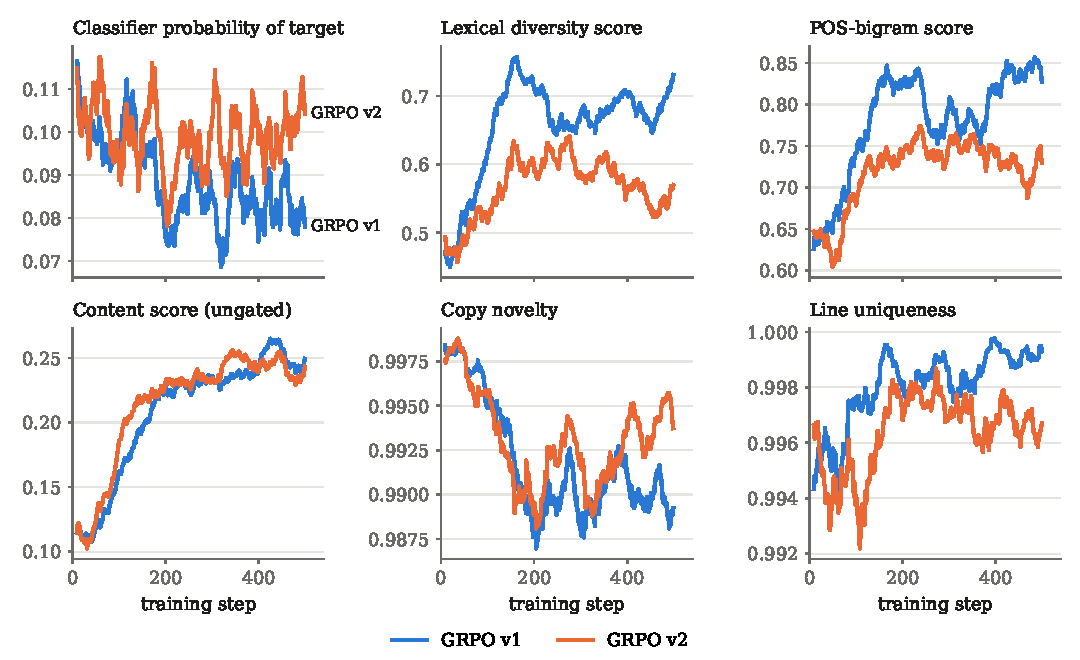
\includegraphics[width=\textwidth]{figures/grpo_training_curves.pdf}
\caption{Reward components during training (mean over the 32 completions per
step, 25-step moving average). Only components on a common scale are shown;
$R$ and the gated terms are not comparable between v1 and v2.}
\label{fig:curves}
\end{figure}

\subsection{GRPO v1}

\paragraph{The reward rose and was not gamed on the gated axes.} v1 beats its
start policy on 94\,\% of the paired items. The content term more than doubles
(0.123 $\to$ 0.302), and degenerate outputs fall from 30.1\,\% to 5.3\,\% under
plain sampling --- matching real poems, from the policy rather than a decoding
control, and with higher rather than lower content recall. The style gain came
from the groups with the largest within-group spread: over training, lexical
diversity rose 0.49 $\to$ 0.71 and POS bigrams 0.64 $\to$ 0.84, while the
classifier term \emph{fell}, 0.102 $\to$ 0.078 (Figure~\ref{fig:curves}).

\paragraph{Author identification went down.} Classifier top-1 fell from 0.158
to 0.079, mostly on Конески and Славеј; the share of outputs read as Конески
fell from 36\,\% to 22\,\%, so v1 partly undid the collapse onto the majority
voice but did not replace it with the requested ones. The judge falls less
(0.158 $\to$ 0.130): a larger loss on the rewarded classifier than on an
independent one is the opposite of gaming, but neither shows a gain.

\paragraph{Partial copying.} Outputs with at least one near-copied source line
rose from 8\,\% to 44\,\%. The gate charges one copied line in twenty only
5\,\% of the content reward, which a gain in line-level F1 can outweigh;
outputs with a copied line have content recall 0.382, those without 0.302.
Checkpoint 300 confirms that later steps trade along this frontier: lower $R$
(0.381) and recall (0.306), less copying (39\,\%), same identification.

\subsection{GRPO v2}

v2 targets both failures: the classifier group is weighted by
$0.288/0.051\approx5.6$, giving it the same pull on the advantage as lexical
diversity and POS bigrams, and the copy gate is cubed, so one copied line in
twenty costs 14\,\% instead of 5\,\%.

\paragraph{The classifier was not gamed.} The judge moves with the reward
classifier, by less (classifier 0.079 $\to$ 0.135, judge 0.130 $\to$ 0.150),
and agrees on 57\,\% of the outputs the reward classifier attributes to the
target, against 62\,\% for SFT and 64\,\% for the teacher.

\paragraph{It held the majority voices rather than learning new ones.} During
training v2's classifier term stays flat (0.106 $\to$ 0.103) where v1's fell:
the weight stopped the policy drifting away from the voices it had, but did not
move it towards the requested ones. Almost all of v2's difference from v1 is
on Конески (0.404 $\to$ 0.638) and Славеј (0.186 $\to$ 0.442), and 36\,\% of
outputs are again read as Конески, the SFT level. The other eight targets stay
at 0--9\,\% on both classifiers. Neither GRPO run beats SFT on author
identification by either measure.

\paragraph{Costs.} With the classifier at 5.6, the share of the style reward
held by lexical diversity and POS bigrams falls from 2/6 to 2/10.6; they rise
far less in training (0.48 $\to$ 0.56 and 0.63 $\to$ 0.72) and degenerate
outputs return to 25\,\%. The cubed gate cut copying (44\,\% $\to$ 34\,\% of
outputs) and with it content recall (0.338 $\to$ 0.270). By the neutral reward
v2 (0.350) is below v1 (0.406), and above it on only 25\,\% of items.

\subsection{Why reweighting cannot fix the collapse}

GRPO's update is driven by differences \emph{within} a group of four samples.
For eight of the ten targets the student's samples are almost never read as
the target by either classifier, before or after GRPO, so all four score near
zero on that term and the normalised advantage has nothing to amplify however
large its weight. The only targets where the classifier term varies within a
group are those the student already writes like, and that is where both runs
moved. The teacher shows the voices are reachable --- judge top-1 0.506, 76\,\%
of the real-poem ceiling, with eight of the ten targets at 0.24 or above --- but that capacity
did not survive distillation into a 4B student from 1{,}146 examples. For GRPO
to help, the student's SFT distribution must already put some probability on
the minority voices.

The teacher also shows what the reward does not measure. Its $R$ (0.395) is
below v1's (0.406): it wins style by a wide margin (0.686 vs.\ 0.511) but
writes a new poem on the source's theme rather than carrying its lines over,
and the line-level content reward scores that barely above an unrelated poem.

% ═══════════════════════════════════════════════════════════════════════════
\section{Status and next steps}\label{sec:next}

\begin{itemize}\itemsep2pt
  \item \textbf{Test split.} All numbers above are on the val split, which was
    also used to make decisions (decoding, v2's reward). The final evaluation
    on the untouched test split --- base, SFT, GRPO v1 and v2 on 466 (test
    poem, target) pairs with the same protocol --- is running
    (\texttt{slurm/eval\_test.slurm}) and will replace these as the reported
    figures.
  \item \textbf{Second student.} The same SFT and GRPO-v2 pipeline is being
    run with Gemma~4 E4B, a student of matched size from the teacher's own
    family, to separate properties of Qwen3-4B from properties of the method.
    It will be reported, and compared with these results, separately.
  \item \textbf{Human evaluation.} A blind rating by native speakers
    (language, coherence, poetic quality, faithfulness to the source, author
    attribution, usability) is planned, with the target's own closest real
    poem as a retrieval baseline.
\end{itemize}

\paragraph{Limitations.} One seed per run, so differences of a few points
(e.g.\ classifier top-1 0.079 vs.\ 0.088 between v1's checkpoints) are within
noise. The reward classifier and TF-IDF palettes were fitted on the whole
corpus, a leak path the judge avoids. SFT had no held-out loss, so the number
of epochs was not validated, and 6.2\,\% of its examples were truncated. The
content signal is narrow: unrelated poems reach line-F1 0.553, and the teacher
itself preserves little content. Author identity is measured automatically
only.

{\raggedright\paragraph{Reproducibility.} Splits: \texttt{make\_splits.py}. Teacher data:
\texttt{generate\_synthetic\_parallel.sh}. SFT, GRPO and evaluation:
\texttt{slurm/train\_sft.slurm}, \texttt{train\_grpo.slurm},
\texttt{train\_grpo\_v2.slurm}, \texttt{eval\_grpo.slurm}. Tables:
\texttt{compare\_generations.py} with \texttt{--rewards} and
\texttt{--corpus-reference} over the tracked
generation CSVs in \texttt{data/validation\_generations/}, which reproduces
every number on CPU. Figure~\ref{fig:curves}:
\texttt{scripts/plot\_grpo\_curves.py}. Every training run records its
arguments, commit, merge provenance and library versions in
\texttt{run\_config.json}.\par}

\end{document}
